\chapter{TINJAUAN PUSTAKA}
\label{chap:tinjauanpustaka}

% Ubah bagian-bagian berikut dengan isi dari tinjauan pustaka

\section{Penelitian Terdahulu}
\label{sec:penelitianterdahulu}

\subsection{Kontrol Kursi Roda Menggunakan Sinyal Suara Melalui Bluetooth}

Pada tahun 2023 telah dilakukan penelitian yang berjudul "Kontrol Kursi Roda Menggunakan Sinyal Suara Melalui Bluetooth" oleh Arief Wisaksono, Rachmad Aditya Pratama, dan Hindarto hindarto dari Departemen Teknik Elektro, Fakultas Sains dan Teknologi Universitas Muhammadiyah Sidoarjo \parencite{wisaksono2023kontrol}.

Pada penelitian ini dapat disimpulkan bahwa pengujian koneksi Bluetooth dan Android dapat berjalan secara optimal. Sehingga input dari Android bisa terkirim ke rangkaian Arduino Uno. Hasil pengujian koneksi memiliki waktu delay selama 4 detik hingga 6 detik. Pengujian baterai 12 Volt memiliki deviasi sebesar 0,43 serta akurasi sebesar 96,7\%. Hal ini disebabkan karena hasil dari pengukuran lebih besar daripada tegangan yang diperlukan. Akan tetapi hal tersebut tidak mempengaruhi sistem kerja alat karena tegangan 12 Volt merupakan tegangan minimum alat.

\subsection{Rancang Bangun Kursi Roda Elektrik Dengan Sistem Kontrol \emph{Joystick} Dan \emph{Smartphone} Android}

Pada tahun 2023 telah dilakukan penelitian yang berjudul "Rancang Bangun Kursi Roda Elektrik Dengan Sistem Kontrol \emph{Joystick} dan \emph{Smartphone} Android" oleh Bayu Ahityanto Wi-caksono dari Program Studi Diploma IV Rekayasa Perancangan Mekanik, Sekolah Vokasi Universitas Diponegoro \parencite{wicaksono2023rancang}.

Pada penelitian ini didapatkan kesimpulan bahwa kursi roda konvensional yang dijadikan kursi roda elektrik berhasil dijalankan dengan kecepatan maksimal 2 km/h sesuai perencanaan. Kursi roda elektrik dapat dikontrol dengan \emph{joystick} maupun dari aplikasi yang berada di \emph{smartphone} android. Kursi roda elektrik dapat berjalan dengan beban maksimal 80 kg. Terdapat beberapa saran dari penulis seperti menambahkan sandaran kepala agar pengguna lebih nyaman di kursi roda elektrik, serta pembuatan sistem aplikasi untuk pengguna \emph{smartphone} dari Apple.

\subsection{\emph{Wheelchair Control Using Bluetooth-Based Electromyography Signals}}

Telah dilakukan penelitian yang berjudul \emph{"Wheelchair Control Using Bluetooth-Based Electromyography Signals"} oleh Yoga Eko Prasetyo dari Program Studi Teknik Elektro dan Hindarto Hindarto dari Program Studi Informatika Universitas Muhammadiyah Sidoarjo \parencite{prasetyo2023wheelchair}.

Pada penelitian ini didapatkan kesimpulan bahwa durasi tunggu dari bluetooth master dengan bluetooth slave sebesar 4 detik hingga 5 detik. Pengujian sensor elektromiografi dapat berjalan dengan normal dan menghasilkan nilai yang berbeda ketika otot berkontraksi maupun relaksasi. 

\subsection{Prototipe Kursi Roda Elektrik Dengan Kendali \emph{Joystick} dan \emph{Smartphone}}

Pada tahun 2019 telah dilakukan penelitian yang berjudul "Prototipe Kursi Roda Elektrik Dengan Kendali \emph{Joystick} dan \emph{Smartphone}" oleh Andy Sadewa Junior dan Fatchul Arifin dari Program Studi Teknik Elektronika, Fakultas Teknik Universitas Negeri Yogyakarta \parencite{junior2019prototipe}.

Pada penelitian ini didapatkan kesimpulan bahwa total \emph{error} yang dihasilkan dari pengujian tegangan motor kiri dan kanan adalah sebesar 0,144\% dan rata-rata \emph{error} yang didapatkan adalah sebesar 0,024\% pada keseluruhan pengujian yang dilakukan. Pada pengujian bluetooth didapatkan kesimpulan bahwa jangkauan pengiriman optimal dari bluetooth apabila tidak ada penghalang adalah sebesar 1 meter hingga 10 meter.

\subsection{\emph{Vision-based Head Posture Control Wheelchair System Research}}

Pada tahun 2023 telah dilakukan penelitian yang berjudul \emph{"Vision-based Head Posture Control Wheelchair System Research"} oleh Pengyu Gao dari \emph{School of Information Engineering}, \emph{Shenyang University of Chemical Technology} bersama Haitao Luo dan Yuxin Li dari \emph{Department of Space Automation Technology}, \emph{Shenyang Institute of Automation}, \emph{Chinese Academy of Sciences} \parencite{10280784}.

Pada penelitian ini didapatkan kesimpulan bahwa sistem pendeteksi pose kepada berbasis Mediapipe berhasil dilakukan menggunakan metode pemodelan matematis yang dikombinasikan dengan fungsi trigonometri untuk memperkirakan sudut wajah dan arah pose kepala. Namun masih terdapat beberapa \emph{error} pada pengenalan citra karena transmisi input citra bersifat \emph{realtime}.

\section{Teori/Konsep Dasar}

\subsection{\emph{Pulse Width Modulation} (PWM)}

\emph{Pulse Width Modulation}, atau PWM, adalah teknik untuk menghasilkan sinyal analog menggunakan metode digital \parencite{Hirzel_2024}. Dalam metode ini, kontrol digital digunakan untuk menghasilkan sinyal yang beralih antara kondisi \emph{on} dan \emph{off}. Sinyal ini kemudian dapat disesuaikan untuk mensimulasikan tegangan di antara nilai VCC penuh (misalnya, 5V pada \emph{board} Arduino UNO, atau 3.3 V pada \emph{board} MKR) dan VCC rendah (0V) dengan mengatur proporsi waktu sinyal dalam kondisi \emph{on} dan \emph{off}. Durasi sinyal dalam kondisi hidup disebut sebagai lebar pulsa (\emph{pulse widht}). Untuk mendapatkan nilai analog yang bervariasi, lebar pulsa tersebut dapat diubah atau dimodulasi. Misalnya, dengan mengulangi pola \emph{on-off} dengan cepat pada sebuah LED, hasilnya akan terlihat seperti tegangan yang stabil antara 0V dan VCC yang mengatur kecerahan LED tersebut.

Pada Gambar \ref{fig:PulseWidthModulation} garis hijau mewakili periode waktu yang teratur. Durasi atau periode ini adalah kebalikan dari frekuensi PWM. Dengan kata lain, dengan frekuensi PWM Arduino sekitar 500HZ maka garis hijau akan memiliki panjang 2 milidetik setiap satunya. Pemanggilan analogWrite() berkisar antara 0-255, sehingga analogWrite(255) akan meminta siklus tugas 100\%(selalu menyala) dan analogWrite(127) akan meminta siklus tugas 50\% (menyala setengah waktu).

\begin{figure} [ht] \centering
    % Nama dari file gambar yang diinputkan
    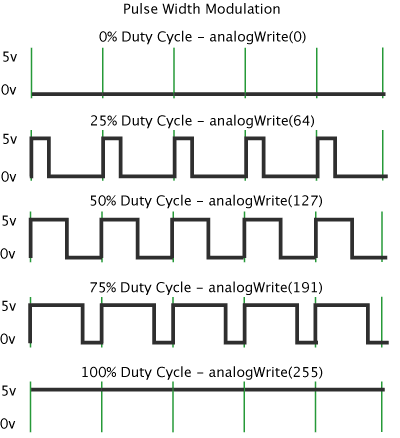
\includegraphics[scale=0.8]{gambar/pwm.png}
    % Keterangan gambar yang diinputkan
    \caption{\emph{Pulse Width Modulation}(PWM)}
    % Label referensi dari gambar yang diinputkan
    \label{fig:PulseWidthModulation}
\end{figure}

\newpage

Pada beberapa mikrokontroler, PWM hanya tersedia pada pin tertentu. Silakan pertimbangkan diagram \emph{pinout} pada \emph{board} yang akan digunakan untuk mengetahui pin mana saja yang dapat digunakan sebagai PWM. Pin yang dapat digunakan sebagai PWM biasanya dilambangkan dengan tanda tilde (\(\sim \)).

\subsection{JSON}

\emph{JavaScript Object Notation} (JSON) merupakan format pertukaran data yang ringan dan mudah digunakan \parencite{Data}. JSON mudah dipahami oleh manusia dan mesin. JSON didasarkan pada sebagian kecil dari Standar Bahasa Pemrograman JavaScript ECMA-262 Edisi ke-3 yang dirilis pada bulan Desember 1999. JSON menggunakan konvensi yang familiar bagi para programmer dengan berbagai latar bahasa pemrograman, termasuk C, C++, C\#, Java, JavaScript, Perl, hingga Python \parencite{Org_2017}. Karena sifatnya yang fleksibel ini membuat JSON menjadi bahasa pertukaran data yang sangat ideal.

JSON terdiri dari 2 struktur utama, yaitu \emph{key} dan \emph{value}. Sekumpulan \emph{key-value} dapat dianggap sebagai objek pada beberapa bahasa pemrograman. Selain itu JSON juga dapat terdiri dari sebuah daftar nilai yang diurutkan (\emph{ordered list of values}). Struktur ini dapat diwakili sebagai \emph{array, vector, list,} maupun \emph{sequence} pada berbagai bahasa pemrograman.

\subsection{Bluetooth}

Bluetooth merupakan sebuah standar terbuka untuk konektivitas nirkabel dengan dukungan tinggi dari industri komputer dan perangkat seluler \parencite{sairam2002bluetooth}. Bluetooth diciptakan pada tahun 1994 oleh L. M. Ericsson dari Swedia. 

Bluetooth Classic radio, juga dikenal sebagai Bluetooth Basic Rate/Enhanced Data Rate (BR/EDR), adalah jenis radio dengan konsumsi daya rendah yang mengirimkan data melalui 79 saluran di band frekuensi 2.4 GHz yang tidak berlisensi untuk penggunaan industri, ilmiah, dan medis (ISM) \parencite{SIG_2024}. Fitur komunikasi antar-perangkat titik ke titik, Bluetooth Classic umumnya digunakan untuk mengaktifkan streaming audio nirkabel dan telah menjadi standar protokol radio untuk perangkat seperti speaker nirkabel, headphone, dan sistem hiburan di mobil. Selain itu, radio Bluetooth Classic juga memungkinkan aplikasi transfer data, termasuk pencetakan melalui perangkat seluler.

Radio Bluetooth Low Energy (BLE) dirancang untuk beroperasi dengan sangat efisien dalam penggunaan daya. Dengan mentransmisikan data melalui 40 saluran di band frekuensi ISM 2.4 GHz yang tidak berlisensi, radio Bluetooth LE memberikan fleksibilitas yang besar bagi para pengembang untuk membuat produk yang sesuai dengan kebutuhan konektivitas pasar mereka. Bluetooth LE mendukung berbagai topologi komunikasi, mulai dari titik ke titik hingga siaran dan, yang terbaru, mesh, sehingga teknologi Bluetooth dapat mendukung pembuatan jaringan perangkat yang andal dan luas. Awalnya dikenal karena kemampuannya dalam komunikasi perangkat, Bluetooth LE kini juga banyak digunakan sebagai teknologi penentuan posisi perangkat untuk mengatasi permintaan yang semakin meningkat untuk layanan lokasi dalam ruangan yang akurat. Bluetooth LE sekarang dilengkapi dengan fitur yang memungkinkan satu perangkat menentukan keberadaan, jarak, dan arah perangkat lainnya. Perbandingan antara Bluetooth Low Energy dengan Bluetooth Classic dapat dilihat pada Tabel \ref{tbl:perbandinganBLEBC}

\begin{longtable}{|p{1.7cm}|l|l|l|}
    \caption{Tabel Perbandingan Bluetooth Low Energy dengan Bluetooth Classic}
    \label{tbl:perbandinganBLEBC}\\
    \hline
                                                                        & Bluetooth Low Energy (BLE)                                                                                                                                                                         & Bluetooth Classic                                                                                                        \\ \hline
    \endfirsthead
    %
    \endhead
    %
    Frequency Band                                                      & 2.4 GHz ISM Band                                                                                                                                                                                   & 2.4 GHz ISM band                                                                                                         \\ \hline
    Channels                                                            & \begin{tabular}[c]{@{}l@{}}40 channels with 2 MHz spacing\\ (3 advertising channels/37 data channels)\end{tabular}                                                                                 & 79 channels with 1 MHz spacing                                                                                           \\ \hline
    Channel Usage                                                       & FHSS                                                                                                                                                                                               & FHSS                                                                                                                     \\ \hline
    Modulation                                                          & GFSK                                                                                                                                                                                               & GFSK, $\pi$/4 DQPSK, 8 DPSK                                                                                              \\ \hline
    Data Rate                                                           & \begin{tabular}[c]{@{}l@{}}LE 2M PHY: 2 Mb/s\\ LE 1M PHY: 1 Mb/s\\ LE Coded PHY (S=2): 500 Kb/s\\ LE Coded PHY (S=8): 125 Kb/s\end{tabular}                                                        & \begin{tabular}[c]{@{}l@{}}EDR PHY (8DPSK): 3 Mb/s\\ EDR PHY ($\pi$/4 DQPSK): 2 Mb/s\\ BR PHY (GFSK): 1Mb/s\end{tabular} \\ \hline
    Tx Power*                                                           & $\le$ 100mW (+20 dBm)                                                                                                                                                                              & $\le$ 100mW (+20 dBm)                                                                                                    \\ \hline
    Rx Sensitivity                                                      & \begin{tabular}[c]{@{}l@{}}LE 2M PHY: $\le$ -70 dBm\\ LE 1M PHY: $\le$ -70 dBm\\ LE Coded PHY (S=2): $\le$ -75 dBm\\ LE Coded PHY (S=8): $\le$ -82 dBm\end{tabular}                                & $\le$ -70 dBm                                                                                                            \\ \hline
    Data Transports                                                     & \begin{tabular}[c]{@{}l@{}}Asynchronous Connection-oriented\\ Isochronous Connection-oriented\\ Asynchronous Connectionless\\ Synchronous Connectionless\\ Isochronous Connectionless\end{tabular} & \begin{tabular}[c]{@{}l@{}}Asynchronous Connection-oriented\\ Synchronous Connection-oriented\end{tabular}               \\ \hline
    \begin{tabular}[c]{@{}l@{}}Commu\\nication \\ Topologies\end{tabular} & \begin{tabular}[c]{@{}l@{}}Point-to-Point (including piconet)\\ Broadcast\\ Mesh\end{tabular}                                                                                                      & Point-to-Point (including piconet)                                                                                       \\ \hline
    \begin{tabular}[c]{@{}l@{}}Positioning \\ Features\end{tabular}     & \begin{tabular}[c]{@{}l@{}}Presence: Advertising\\ Direction: Direction Finding(AoA/AoD)\\ Distance: RSSI, HADM(Coming)\end{tabular}                                                               & None                                                                                                                     \\ \hline
\end{longtable}

\subsection{WiFi}

WiFi merupakan teknologi jaringan nirkabel yang dapat menghubungkan perangkat dengan perangkat lainnya maupun terhubung dengan internet. WiFi terstandarisasi sebagai IEEE 802.11. Keuntungan terbesar dari WiFi adalah kesederhanaannya. Komputer dapat dihubungkan tanpa kabel baik dengan internet maupun dengan perangkat lainnya. Komputer terhubung ke jaringan menggunakan sinyal radio dengan radius sejauh 100 kaki. 

Radio WiFi yang bekerja pada standar 802.11b dan 802.11g mengirimkan sinyal pada frekuensi 2.4GHz, sementara WiFi dengan standar 802.11a mengirimkan sinyal pada frekuensi 5GHz. Frekuensi yang lebih tinggi akan memungkinkan pengiriman data yang lebih tinggi.

Radio WiFi menggunakan teknik pengkodean yang jauh lebih efisien. Untuk standar 802.11a dan 802.11 g, teknik ini dikenal sebagai \emph{Orthogonal Frequency-Division Multiplexing}(OFDM). Sedangkan untuk standar 802.11b, teknik ini disebut \emph{Complementary Code Keying}(CCK).

Kartu WiFi 802.11b memiliki kemampuan untuk mentransmisikan sinyal pada tiga frekuensi yang berbeda secara langsung. 802.11b juga dapat membagi lebar pita radio yang tersedia menjadi banyak saluran dan dengan cepat berpindah-pindah frekuensi diantara mereka. Metode ini lebih tahan terhadap gangguan dan dapat memungkinkan banyak kartu WiFi beroperasi secara bersamaan tanpa saling mengganggu.

Radio WiFi dapat mengirimkan data yang besar pada setiap detiknya. Standar 802.11b dapat menangani hingga 11 Mb/detik. Sedangkan standar 802.11a dan 802.11g mampu menangani hingga 54 Mb/detik.

\emph{The Instituteof Electrical and Electronics Engineers} (IEEE) telah membuat standar penamaan dan penomoran yang unik pada teknologi WiFi. Standar 802.11 berkaitan erat dengan jaringan nirkabel. Notasi a, b, dan g mengidentifikasikan variasi yang berbeda dari standar 802.11. 

\subsection{Arduino IDE}

Arduino Integrated Development Environment (IDE) merupakan perangkat lunak sumber terbuka yang digunakan untuk menulis dan mengunggah kode ke mikrokontroler seperti Arduino maupun ESP buatan Espressif System. Arduino IDE berisikan editor teks untuk menulis kode program, toolbar dengan tombol untuk fungsi umum serta serangkaian menu. Program yang ditulis menggunakan Arduino IDE disebut sketches. Sketches ditulis 
pada teks editor dan disimpan pada file dengan ekstensi .ino. Editor memiliki fitur untuk memotong dan menempel serta untuk mencari dan mengganti teks. Area pesan akan memberikan umpan balik ketika menyimpan dan mengekspor serta akan menampilkan error. Konsol menampilkan keluaran teks oleh Arduino IDE termasuk pesan error yang lengkap serta informasi lainnya \parencite{Söderby_Hylén_2023a}.

\begin{figure} [ht] \centering
    % Nama dari file gambar yang diinputkan
    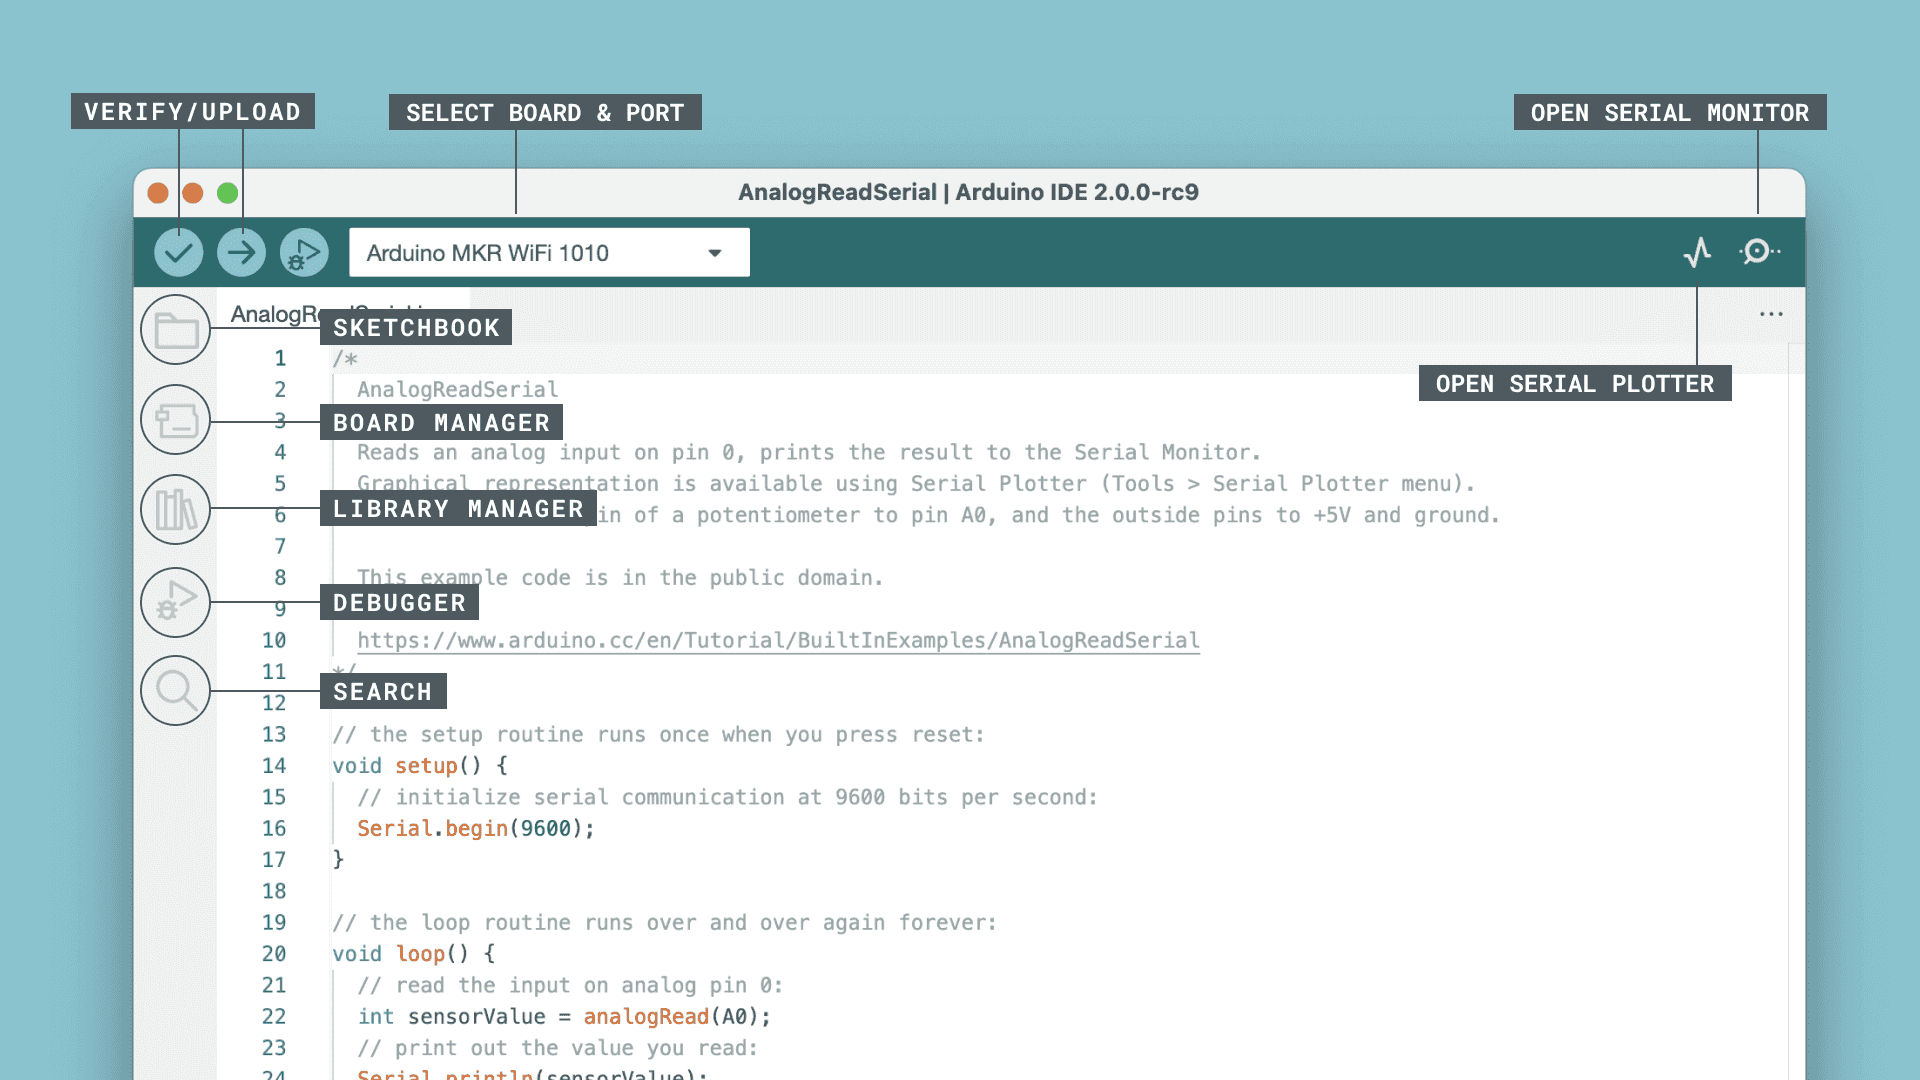
\includegraphics[scale=0.235]{gambar/arduinoIDEoverview.png}
    % Keterangan gambar yang diinputkan
    \caption{Tampilan Arduino IDE 2}
    % Label referensi dari gambar yang diinputkan
    \label{fig:ArduinoIDEOverview}
\end{figure}

Gambar \ref{fig:ArduinoIDEOverview} merupakan tampilan dari Arduino IDE. Arduino IDE 2 dilengkapi dengan \emph{sidebar} baru yang memudahkan pengguna dalam mengakses \emph{tools} yang umum digunakan. \emph{Verify/Upload} digunakan untuk \emph{compile} dan \emph{upload} program ke \emph{Board} Arduino. \emph{Select Board} \& \emph{Port} digunakan untuk mendeteksi \emph{Board} Arduino beserta nomor port yang terhubung dengan Arduino. \emph{Sketchbook} merupakan tempat untuk mencari semua \emph{sketchbook} lokal yang disimpan pada komputer pengguna. Sebagai tambahan, pengguna dapat menguhubungkan Arduino IDE dengan Arduino Cloud sehingga pengguna dapat menyimpan \emph{sketch} pada lingkungan daring. \emph{Board Manager} merupakan kumpulan \emph{board} arduino serta \emph{board packages} pihak ketiga yang dapat diinstal \parencite{Söderby_Hylén_2023b}. \emph{Library Manager} merupakan tempat untuk menginstal berbagai \emph{library} yang mendukung pengembangan Arduino, baik yang dibuat oleh Arduino maupun dari komunitas \parencite{Söderby_Hylén_2023c}. \emph{Debugger} berguna untuk menguji dan men-\emph{debug} program secara \emph{realtime}. \emph{Search} digunakan untuk mencari kata kunci pada program yang sedang dimuat. \emph{Open Serial Monitor} berguna untuk memuat Serial Monitor yang sangat berguna untuk pengembangan \parencite{Söderby_2023}.

\emph{Sketchbook} merupakan tempat dimana file program akan disimpan. \emph{Sketches} Arduino akan disimpan dengan tipe file .ino dan harus disimpan pada folder dengan nama folder yang sama dengan nama file. Sebagai contoh, file my\_sketch.ino harus disimpan pada folder dengan nama folder my\_sketch.

Dengan menggunakan \emph{Library Manager}, pengguna dapat menemukan dan menginstal ribuan \emph{library} yang dapat membantu dalam mengembangkan proyek menggunakan . \emph{Library} merupakan \emph{extension} dari Arduino API yang dapat memudahkan pengembang. Sebagai contoh, para pengembang dapat mengontrol motor servo, membaca sensor tertentu, hingga menggunakan modul WiFi hanya dengan memanggil fungsi yang terdapat pada \emph{library} \parencite{Söderby_Hylén_2023c}.

\emph{Serial Monitor} merupakan alat yang memungkinkan pengguna untuk melihat \emph{streaming} data pada \emph{Board} Arduino yang terhubung. Pada Arduino versi 1, \emph{tool} ini ditempatkan pada jendela yang terpisah, namun untuk memudahkan pengguna maka \emph{tool} ini kini terintegrasi dengan editor \parencite{Söderby_2023}. 

\subsection{NVIDIA® Jetson Nano™}

\begin{figure} [ht] \centering
    % Nama dari file gambar yang diinputkan
    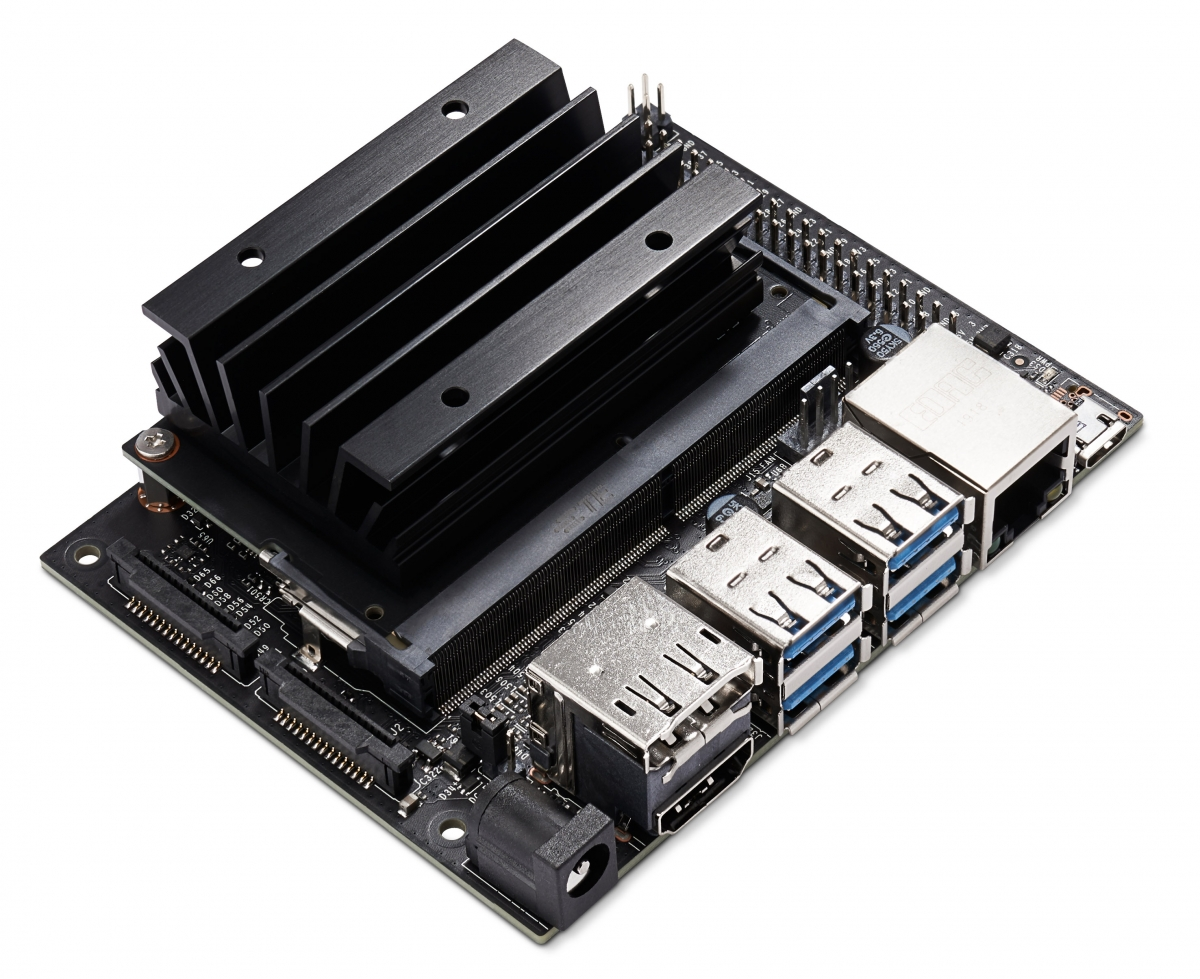
\includegraphics[scale=0.25]{gambar/JetsonNano.jpg}
    % Keterangan gambar yang diinputkan
    \caption{Perangkat Jetson Nano}
    % Label referensi dari gambar yang diinputkan
    \label{fig:Perangkat Jetson Nano}
\end{figure}

NVIDIA® Jetson Nano™ Developer Kit adalah komputer kecil dan kuat yang dapat digunakan untuk menjalankan beberapa \emph{neural network} secara paralel untuk berbagai penerapan seperti klasifikasi gambar, deteksi objek, segmentasi, dan pemrosesan ucapan. Semuanya dikemas dalam platform yang mudah digunakan dan hanya membutuhkan daya 5 watt \parencite{Developer_2023}.

Perangkat ini memiliki pin \emph{input} serta \emph{output} yang berlimpah, mulai dari GPIO hingga pin CSI. Jumlah pin yang berlimpah ini sangat memudahkan para pengembang dalam menghubung-kan berbagai perangkat tambahan seperti sensor untuk keperluan pengembangan aplikasi \emph{Artificial Intelligence}. NVIDIA® Jetson Nano™ Developer Kit juga didukung dengan NVIDIA JetPack yang mencakup berbagai perangkat lunak seperti Sistem Operasi Linux, cuDNN, NVIDIA CUDA, TensorRT, dan juga \emph{Board Support Package} (BSP) yang digunakan untuk keperluan \emph{Deep Learning} serta visi komputer.

\subsection{ESP32 Devkit V1}

\begin{figure} [ht] \centering
    % Nama dari file gambar yang diinputkan
    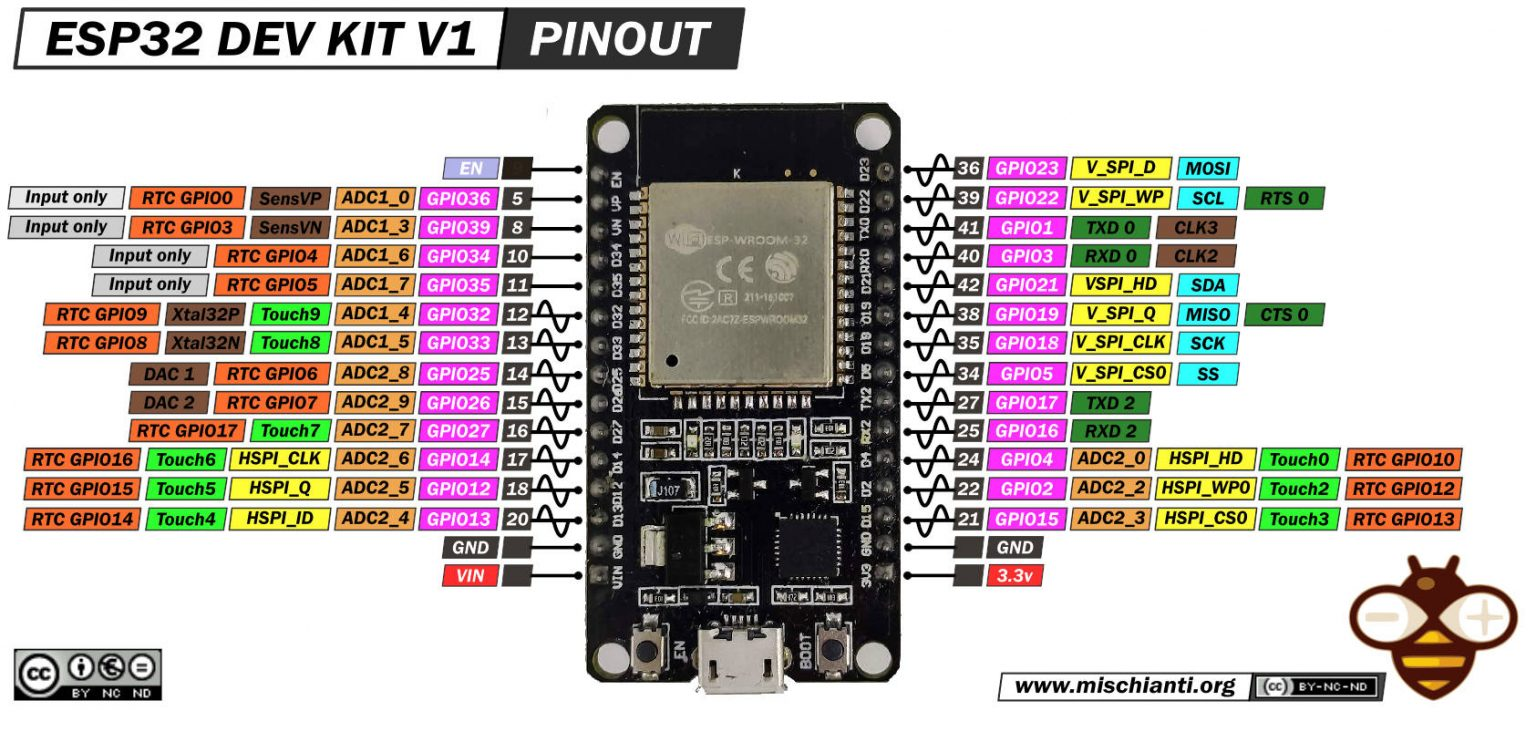
\includegraphics[scale=0.39]{gambar/ESP32DevkitV1.jpg}
    % Keterangan gambar yang diinputkan
    \caption{Perangkat ESP32 Devkit V1}
    % Label referensi dari gambar yang diinputkan
    \label{fig:Perangkat ESP32}
\end{figure}

ESP32 Devkit V1 merupakan salah satu \emph{development board} yang dibuat oleh DOIT untuk menjalankan modul ESP-WROOM-32 buatan Espressif \parencite{SmartArduino_2022}. \emph{Development Board} ini berisi WiFi, Bluetooth, serta berdaya rendah hanya dengan 1 chip. Setiap pin dari ESP32 Devkit V1 dapat dilihat pada Gambar \ref{fig:Perangkat ESP32}. Flash internal modul ESP32 disusun dalam satu area flash dengan 4096 \emph{byte} pada masing-masing halaman. Alamat flash dimulai dari 0x00000.

Daya untuk menjalankan ESP32 disuplai melalui konektor Micro USB Tipe B atau dapat langsung melalui pin "VIN". Perangkat dapat beroperasi pada tegangan antara 6 Volt hingga 20 Volt. Jika menggunakan daya lebih dari 12 Volt maka regulator akan menjadi panas sehingga dapat merusak perangkat.

\subsection{\emph{Motor Driver H-Bridge}}

\emph{H-Bridge} merupakan salah satu jenis \emph{driver motor} yang paling sering digunakan untuk mengendalikan motor listrik. Perangkat ini dapat digunakan untuk mengendalikan arah serta kecepatan putar motor. \emph{Driver Motor H-Bridge} bekerja seperti saklar pada transistor. Transistor merupakan bagian utama dari perangkat ini. \emph{Driver Motor H-Bridge} tersusun oleh sekumpulan transistor yang berfungsi sebagai pengendali motor, terutama yang memerlukan arus serta tegangan yang cukup besar \parencite{Muhammad_2018}.

\begin{figure} [ht]
    \centering
        % Nama dari file gambar yang diinputkan
        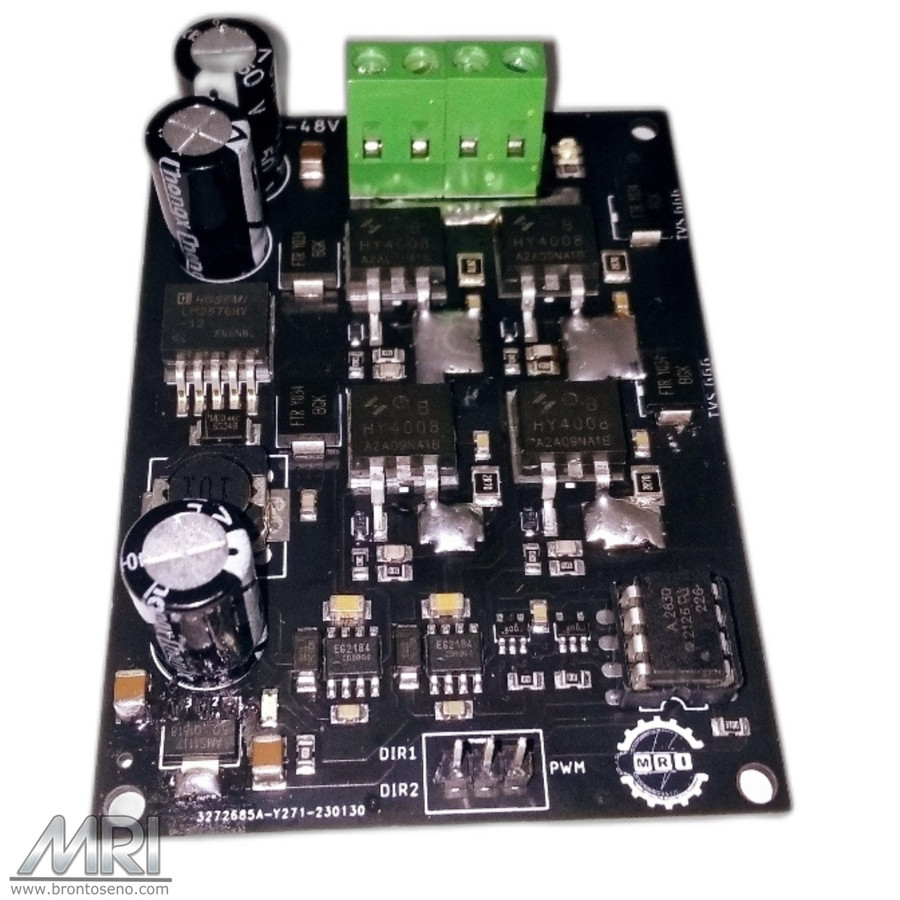
\includegraphics[scale=0.2]{gambar/MotorDriver.png}
        % Keterangan gambar yang diinputkan
        \caption{\emph{H-Bridge Motor Driver}}
        % Label referensi dari gambar yang diinputkan
        \label{fig:DriverMotor}
\end{figure}

Penelitian ini menggunakan \emph{Motor Driver H-Bridge} dari MRI. Perangkat ini dapat digunakan untuk mengatur kecepatan dan arah putar motor \emph{brushed} dengan kapasitas maksimal 50 A pada tegangan 48 V. Driver motor ini dilengkapi dengan satu kanal PWM yang dapat digunakan untuk mengatur kecepatan putar motor dengan cara mengubah lebar pulsa yang dikirimkan ke motor. Lebar pulsa PWM dapat diatur menggunakan potensiometer maupun melalui kontrol sinyal eksternal. Perangkat ini juga memiliki kemampuan untuk mengatur arah putar motor melalui kedua pin dir. Dengan mengganti keadaan \emph{input} kontrol maka pengguna dapat mengubah arah putaran motor secara mudah. Gambar \ref{fig:DriverMotor} merupakan perangkat yang digunakan pada penelitian ini.

\subsection{Kursi Roda Elektrik KY-123}

\begin{figure} [ht]
    \centering
        % Nama dari file gambar yang diinputkan
        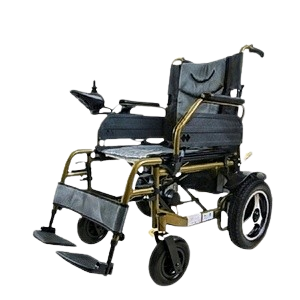
\includegraphics[scale=0.72]{gambar/WheelchairMySellaKY123.png}
        % Keterangan gambar yang diinputkan
        \caption{Kursi Roda Elektrik KY-123}
        % Label referensi dari gambar yang diinputkan
        \label{fig:KY123}
\end{figure}

Kursi roda elektrik sebagian besar terdiri dari rangka kursi roda, alat kontrol gerak kursi roda, motor listrik, serta unit baterai. Alat ini dapat dioperasikan dengan fleksibel, mudah, dan sederhana sehingga tidak memerlukan tenaga yang besar dari pengguna jika dibandingkan dengan kursi roda biasa. Kursi roda ini dapat dioperasikan dengan satu tangan oleh pengguna yang mengalami kelumpuhan hemiplegia. Alat ini juga dapat membantu manula yang susah dalam melakukan mobilisasi. 

Perusahaan MySella telah mengembangkan beberapa model kursi roda elektrik sesuai dengan skenario dan syarat pengaplikasian yang berbeda. Gambar \ref{fig:KY123} merupakan salah satu kursi roda elektrik buatan MySella yang digunakan pada penelitian ini. Kursi roda ini sudah memenuhi persyaratan standar nasional GB 12996-2012. Berikut Tabel \ref{tbl:gb12996} yang menjadi persyaratan standar nasional GB12996-2012.

\begin{longtable}{|l|l|}
    \caption{Standar Nasional GB 12996-2012}
    \label{tbl:gb12996}\\
    \hline
    \multicolumn{1}{|c|}{Parameter} & Indikator Kinerja \\ \hline
    \endfirsthead
    %
    \endhead
    %
    Kecepatan Maksimal              & $\le$ 6 Km/Jam          \\ \hline
    Derajat Kemiringan              & 6\textdegree - 8\textdegree               \\ \hline
    Ketinggian Penghalang           & $\le$ 40 mm             \\ \hline
    Jarak Tempuh                    & $\le$ 20 Km             \\ \hline
    Radius Putar Minimal            & 1.2 m             \\ \hline
    Kemampuan Docking               & 9\textdegree                 \\ \hline
    Lebar Parit                     & 100 mm            \\ \hline
    Suhu Kerja Optimal              & -5\textdegree C - 40\textdegree C           \\ \hline
\end{longtable}

\subsection{Motor DC MY1016Z}

\begin{figure} [ht]
    \centering
        % Nama dari file gambar yang diinputkan
        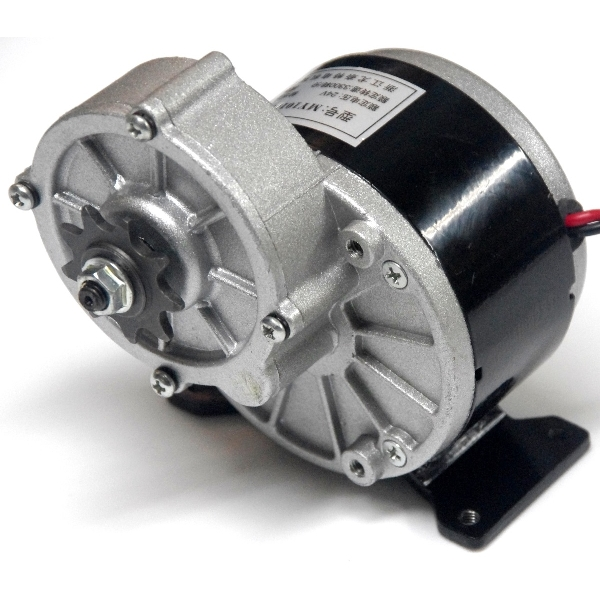
\includegraphics[scale=0.4]{gambar/DCMotorMY1016Z.jpg}
        % Keterangan gambar yang diinputkan
        \caption{Motor DC MY1016Z}
        % Label referensi dari gambar yang diinputkan
        \label{fig:MY1016Z DC Motor}
\end{figure}

Motor DC merupakan jenis dari motor listrik yang menggunakan arus searah untuk menghasilkan gerakan. MY1016Z merupakan \emph{geared} motor DC yang menggunakan mekanisme roda gigi didalamnya. Motor DC ini sering digunakan pada sepeda listrik serta kendaraan sejenisnya. Kursi roda buatan MySella yang bertipe KY-123 juga menggunakan motor DC MY1016Z seperti pada Gambar \ref{fig:MY1016Z DC Motor}.
